Today I should be around for more talks. The day begins with a keynote!

\subsection{Keynote: Pierre-Yves Oudeyer on AI and Education}

{\bf Note:} Children are extraordinary learners! And typically do so without an engineer following them hand tuning every aspect of their learning algorithm and environment. \\

\begin{figure}[h!]
    \centering
    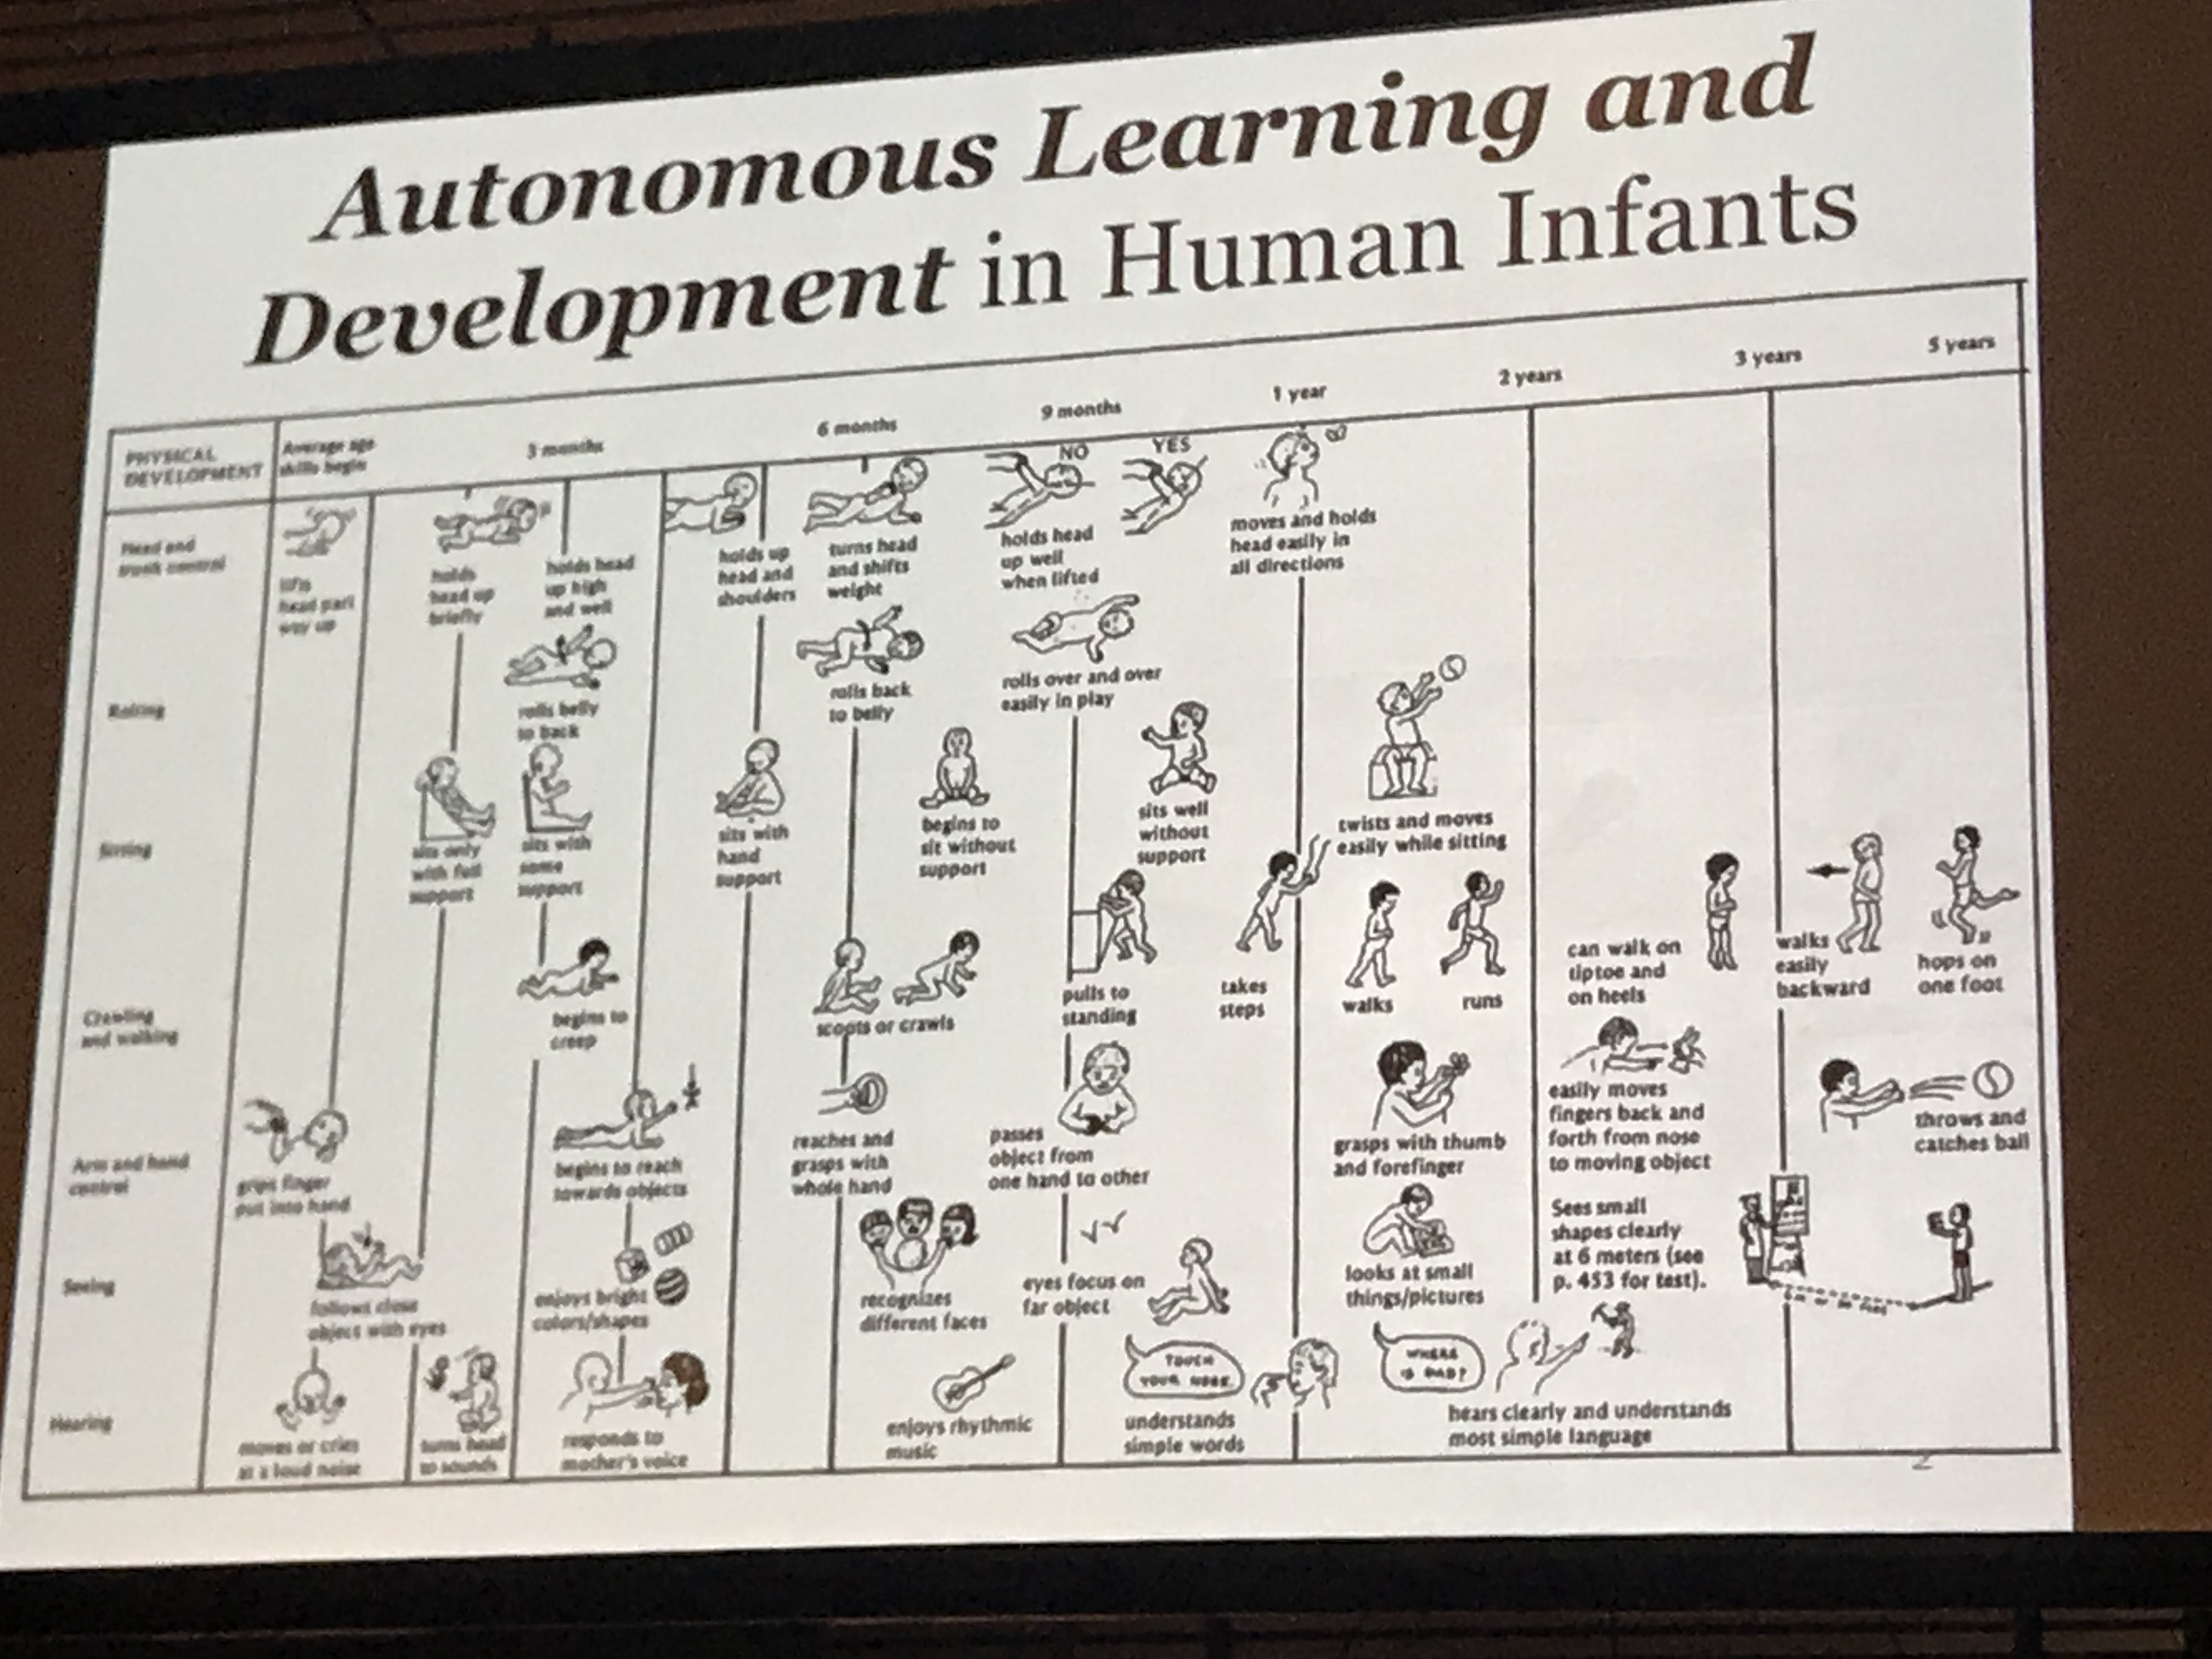
\includegraphics[width=0.4\textwidth]{images/child_learners.JPG}
    \caption{Learning and development in human infants.}
    \label{fig:child learners}
\end{figure}

Guiding Fields:
\begin{enumerate}
    \item {\it Cognitive Science:} Understanding human development and learning
    \item {\it Robotics:} new theory for lifelong and autonomous learning
    \item {\it Applications} in education technology.
\end{enumerate}


Example 1: study of {\it morphology}, body growth, and maturation in designing motor and perceptual primtives in a robot. \\

Example 2: consider language acquisition. Children learn new language very quickly. \\

Example 3: intrinsic motivation, play, and curiosity. \\

Q: How can we understand these practices, and harness them in AI tools, and build new educational tools around them? \\

\subsubsection{Intrinsic Motivation and Curiosity}

Consider {\it active exploration}: video of a baby playing with a variety of toys in a room over time (reminds me of the playroom domain from RL). \\

$\ra$ Similarly, give a baby a few toys, and a hollow cylinder suspended off the ground with a toy car inside of it. The baby over time tends to put the toy into the cylinder which knocks the car out of the tube (at which point the parent is very happy!). \\

$\ra$ But! When the car pops out of the tube, the baby also tends to pick up the car and put it back in the tube. \\

Other children experiment in very {\it different} ways; one kid picked up the block and hit the cylinder to make noises, and seemed very pleased by the noises. This was considered a ``failure" in the study, but was pretty sophisticated exploration! \\

{\bf Note:} Theories of intrinsic motivation, curiosity, and active learning drive to reduce uncertainty, experience novelty, surprise, or challenge. See~\citet{berlyne1960conflict} and~\citet{berlyne1978curiosity}. \\

{\bf Perspective:} The child is a sense making organism: explore to make good predictive models of the world and control it! \\

Q: Based on this perspective, what kind of modeling/algorithms are needed in order to explain these behaviors? \\

A: We use robotic playgrounds -- place robots in a playroom like environment, and encourage them to play to learn object models and affordances. Also place another robot in the playroom that gives ``feedback" (positive/negative reward) to play the role of a parent encouraging/discourgaing the baby.\\

Essential ingredients in these robots:
\begin{itemize}
    \item Dynamic movement primitives
    \item Object-based perceptual primitives (like infants, build on prior perceptual learning)
    \item Self supervised learning forward/inverse models with hindsight learning
    \item Curiositry-driven, self-motivated play and exploration.
\end{itemize}


\subsubsection{The Learning Progress Hypothesis}

Q: What is an {\it interesting} learning experiment for a robot/baby to conduct (to learn)? \\

Lots of answers in the literature: high predictability, high novelty, high uncertainty, knowledge gap, novelty, challenge, surprise, free energy, and so on. \\

{\bf This Work:} The Learning Progress Hypothesis~\cite{oudeyer2016intrinsic}:

\ddef{Learning Progress Hypothesis}{The ``interestingness" of an experiment is directly proportional to empirical learning progress (absolute value of derivative of the errors)}

$\ra$ Few assumptions on underlying learning machinery and on match between biases and real world. \\


{\bf Framework:} suppose we have some robots with motion primitives. Takes some sequence of actions to yield a trajectory:
\[
\tau = (s_t, a_t, s_{t+1}, \ldots).
\]
From this trajectory, the robot should learn, assuming some behavioral abstraction $\phi$:
\begin{enumerate}
    \item Forward model: $F_i : s, \theta \ra \phi_i$, with $\theta$ the parameters of the behavioral policy, $\pi_theta$.
    \item Inverse model: $I_i : s, \phi_i \ra \argmin_\theta ||\phi_i - F_i(s,\theta)||$
\end{enumerate}

Use these two models to measure ``competence progress" as a proxy of the empirical learning progress. \\

$\ra$ Example 1: hierarchical multi-armed bandits. Split a space into subregions, where an agent monitors the errors of each subregion. Use these errors to measure the learning progress over time. Then, in the bandit setting, can explore based on the ratio of these errors over time. \\

$\ra$ Example 2: explore omni-directional locomotion. Look at diversity (in terms of spread of states reached in some space) of outcomes by different exploration policies on a robot. Finding: curiosity-driven exploration is less-efficient than goal exploration.\\

Q: Why is curiosity driven exploration less efficient? \\

A: Forward model exploration (curiosity): knowing many ways to produce a few effects, inverse model exploration (goal): knowing a few ways to produce many effects. \\

Example: curiosity-driven discovery of tool use. Videos of a few robots playing with different tools (a robot with a cup learning to interact with a ball, a gripper robot learning to interact with a joystick). \\

$\ra$ Point: focus on playing with and manipulating objects in the world. The gripper robot learns to manipulate the joysticks, which moves the robot that can pickup the ball. Torso eventually learns to make a light, play a sound, and hide the ball in the cup. \\

Project: ``MUGL: exploring learned modular goal spaces"~\cite{laversanne2018curiosity}. Main idea is to extend these exploration techniques to high dimensional input (the robot examples above used a feature vector, not images). \\

$\ra$ MUGL can be used to discovery independently controllable features (learn to control a ball, and so on).

\subsubsection{Models of Child Development Data}

Experiment: modeling vocal development. Use exact same algorithms from before. \\

$\ra$ Goal: make experiments for the infant using the learning progress idea from before. \\

{\bf Finding:} Some self-organization of developmental structure in infants. First vocal track is learned (unarticulated sounds) and then learns articulated sounds. \\

$\ra$ Observe: regularities that tend to occur at the same time across different individuals, but some things change dramatically. Interactions between learning system and body morphology is stochastic, contingency in exploration, surprising that many things remain constant. \\

\begin{figure}[h!]
    \centering
    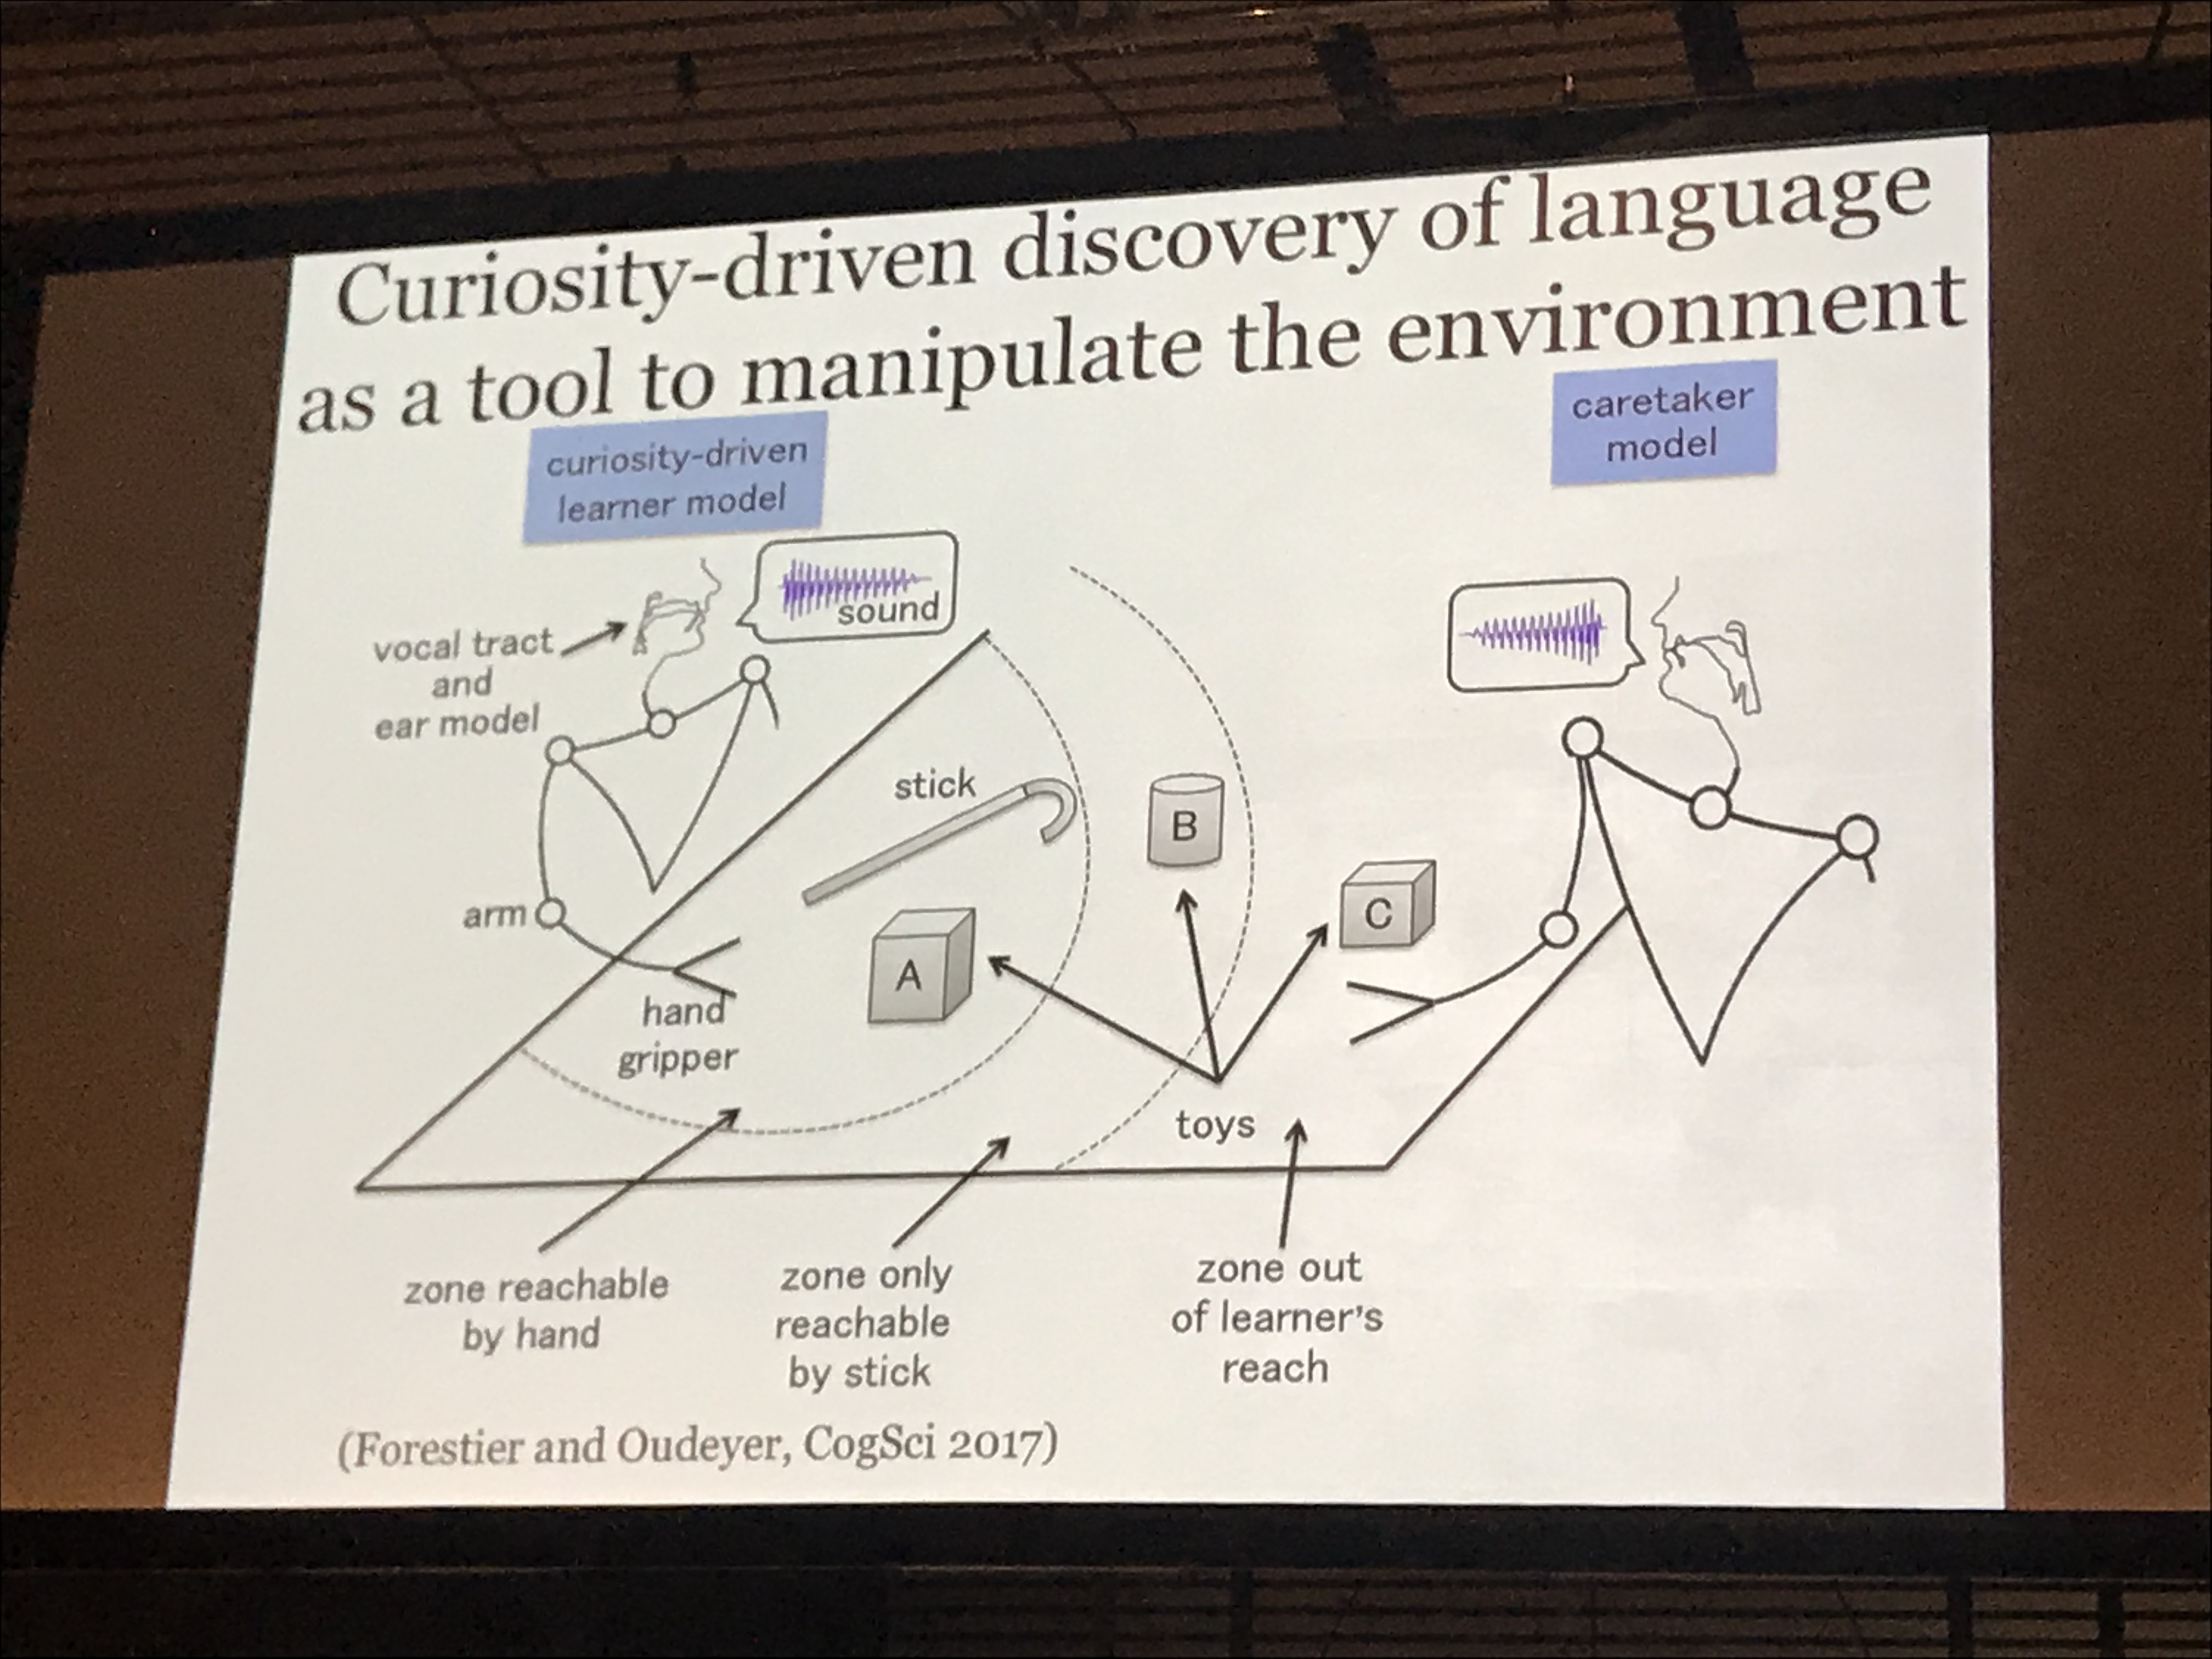
\includegraphics[width=0.4\textwidth]{images/curious.JPG}
    \caption{Curiosity-driven discovery of language}
    \label{fig:curiosity}
\end{figure}

The ``Ergo-Robots" (with Mikhail Gromov and David Lynch, I think?) \dnote{Lynch! :o}. Surreal video of robots learning to speak and interact with their environment and companions, see a sample video here: \url{https://www.youtube.com/watch?v=J0gM5i091JQ}. Robots learn to use language in a meaningful way through exploration. \\

$\ra$ Use similar ideas to come up with a realistic models of learning to use a vocal track. See: {\it Self-Organization in the Evolution of Speech}~\cite{oudeyer2006self}. \\

{\bf Finding:} The distributions of vowels we find in the world languages matches those of the systems that emerge in these curiosity-driven learning systems. This might explain some regularities of language structure. \\




Q: How is spontaneous exploration structured during free play? \\

A: Experiment! Let subjects play a bunch of games/tasks, with no guidelines. Just do whatever you want (play games like guitar hero, free to pick any level/song). \\

$\ra$ People tend to focus on levels of intermediate complexity; exploration follows a controlled growth in complexity, actively controlled by individuals' predictive models. 


\subsubsection{Applications in Educational Technologies}


{\bf Goal:} Develop technologies for fostering efficient learning and intrinsic motivation. \\

$\ra$ Project: KidLearn -- allows personalization of intelligent tutoring systems, based on experiments with $>$ 1000 children in 30+ schools. \\

Principle: graph (usually a DAG) defines difficulty of task/exercise type. This allows the system to sample exercises in some sequence (but still give the kids some choice among nodes in the graph). \\

Main study:
\begin{itemize}
    \item Examine learning impact based on these interventions.
    \item Compare to typical pedagogical expert (vs. their system).
    \item Find that students tend to achieve higher success rate with certain variations of the algorithm.
\end{itemize}

{\bf Takeaways:} Fundamental role of spontenous developmental exploration, can be harnessed to develop human-like robots and empower the learning process.

\subsection{Contributed Talks}
Next up some contributed talks.

\subsubsection{Devon Hjelm on Deep InfoMax~\cite{hjelm2018learning}}

{\bf Broad Goal:} Learn unsupervised image representations. \\

Example: video of a dog catching a snowball. What annotations make sense? (``Cute dog!", ``Good boy!"). \\

$\ra$ Not clear these are the right/useful annotations. \\

{\bf Point:} Don't always want supervised learning of representations. Annotations rarely tell the whole story, real world doesn't come with labels, and really want to find the underlying structure (annotations might not enhance this part). \\

Preliminaries:
\begin{itemize}
    \item Encoder: $E_\psi : \mc{X} \ra Y$, with $Y$ a representation.
    
    \item Mutul info; $I(X;Y) = D_{KL}(P(X,Y) \mid \mid P(x) p(y)$
\end{itemize}

$\ra$ Introduce amutual information estimator: encode an image into a representation. Take pairs of representations from images that aren't associated with each other, and treat these as {\it negative} samples,. \\

{\bf Approach:} 
\begin{enumerate}
    \item Encode input $X$ input $Y$ via $E_\psi$.
    \item Use output to estimate $\hat{I}(X;Y)$, and maximize this estimate.
    \item Just doing this alone isn't quite enough.
    
    {\it Intuition:} you might not pick up on the relevant locations of an image. Consider a picture of a cat, the background isn't as crucial as the information in the front.
    
    \item So: instead of maximizing the mutual info globally, instead maximize it {\it locally}. Perform this estimation/maximization across all locations simultaneously. See Figure~\ref{fig:cat}
    \item This yields local feature vectors for different regions of the image, which can then be stitched together into a global feature vector.
\end{enumerate}

\begin{figure}
    \centering
    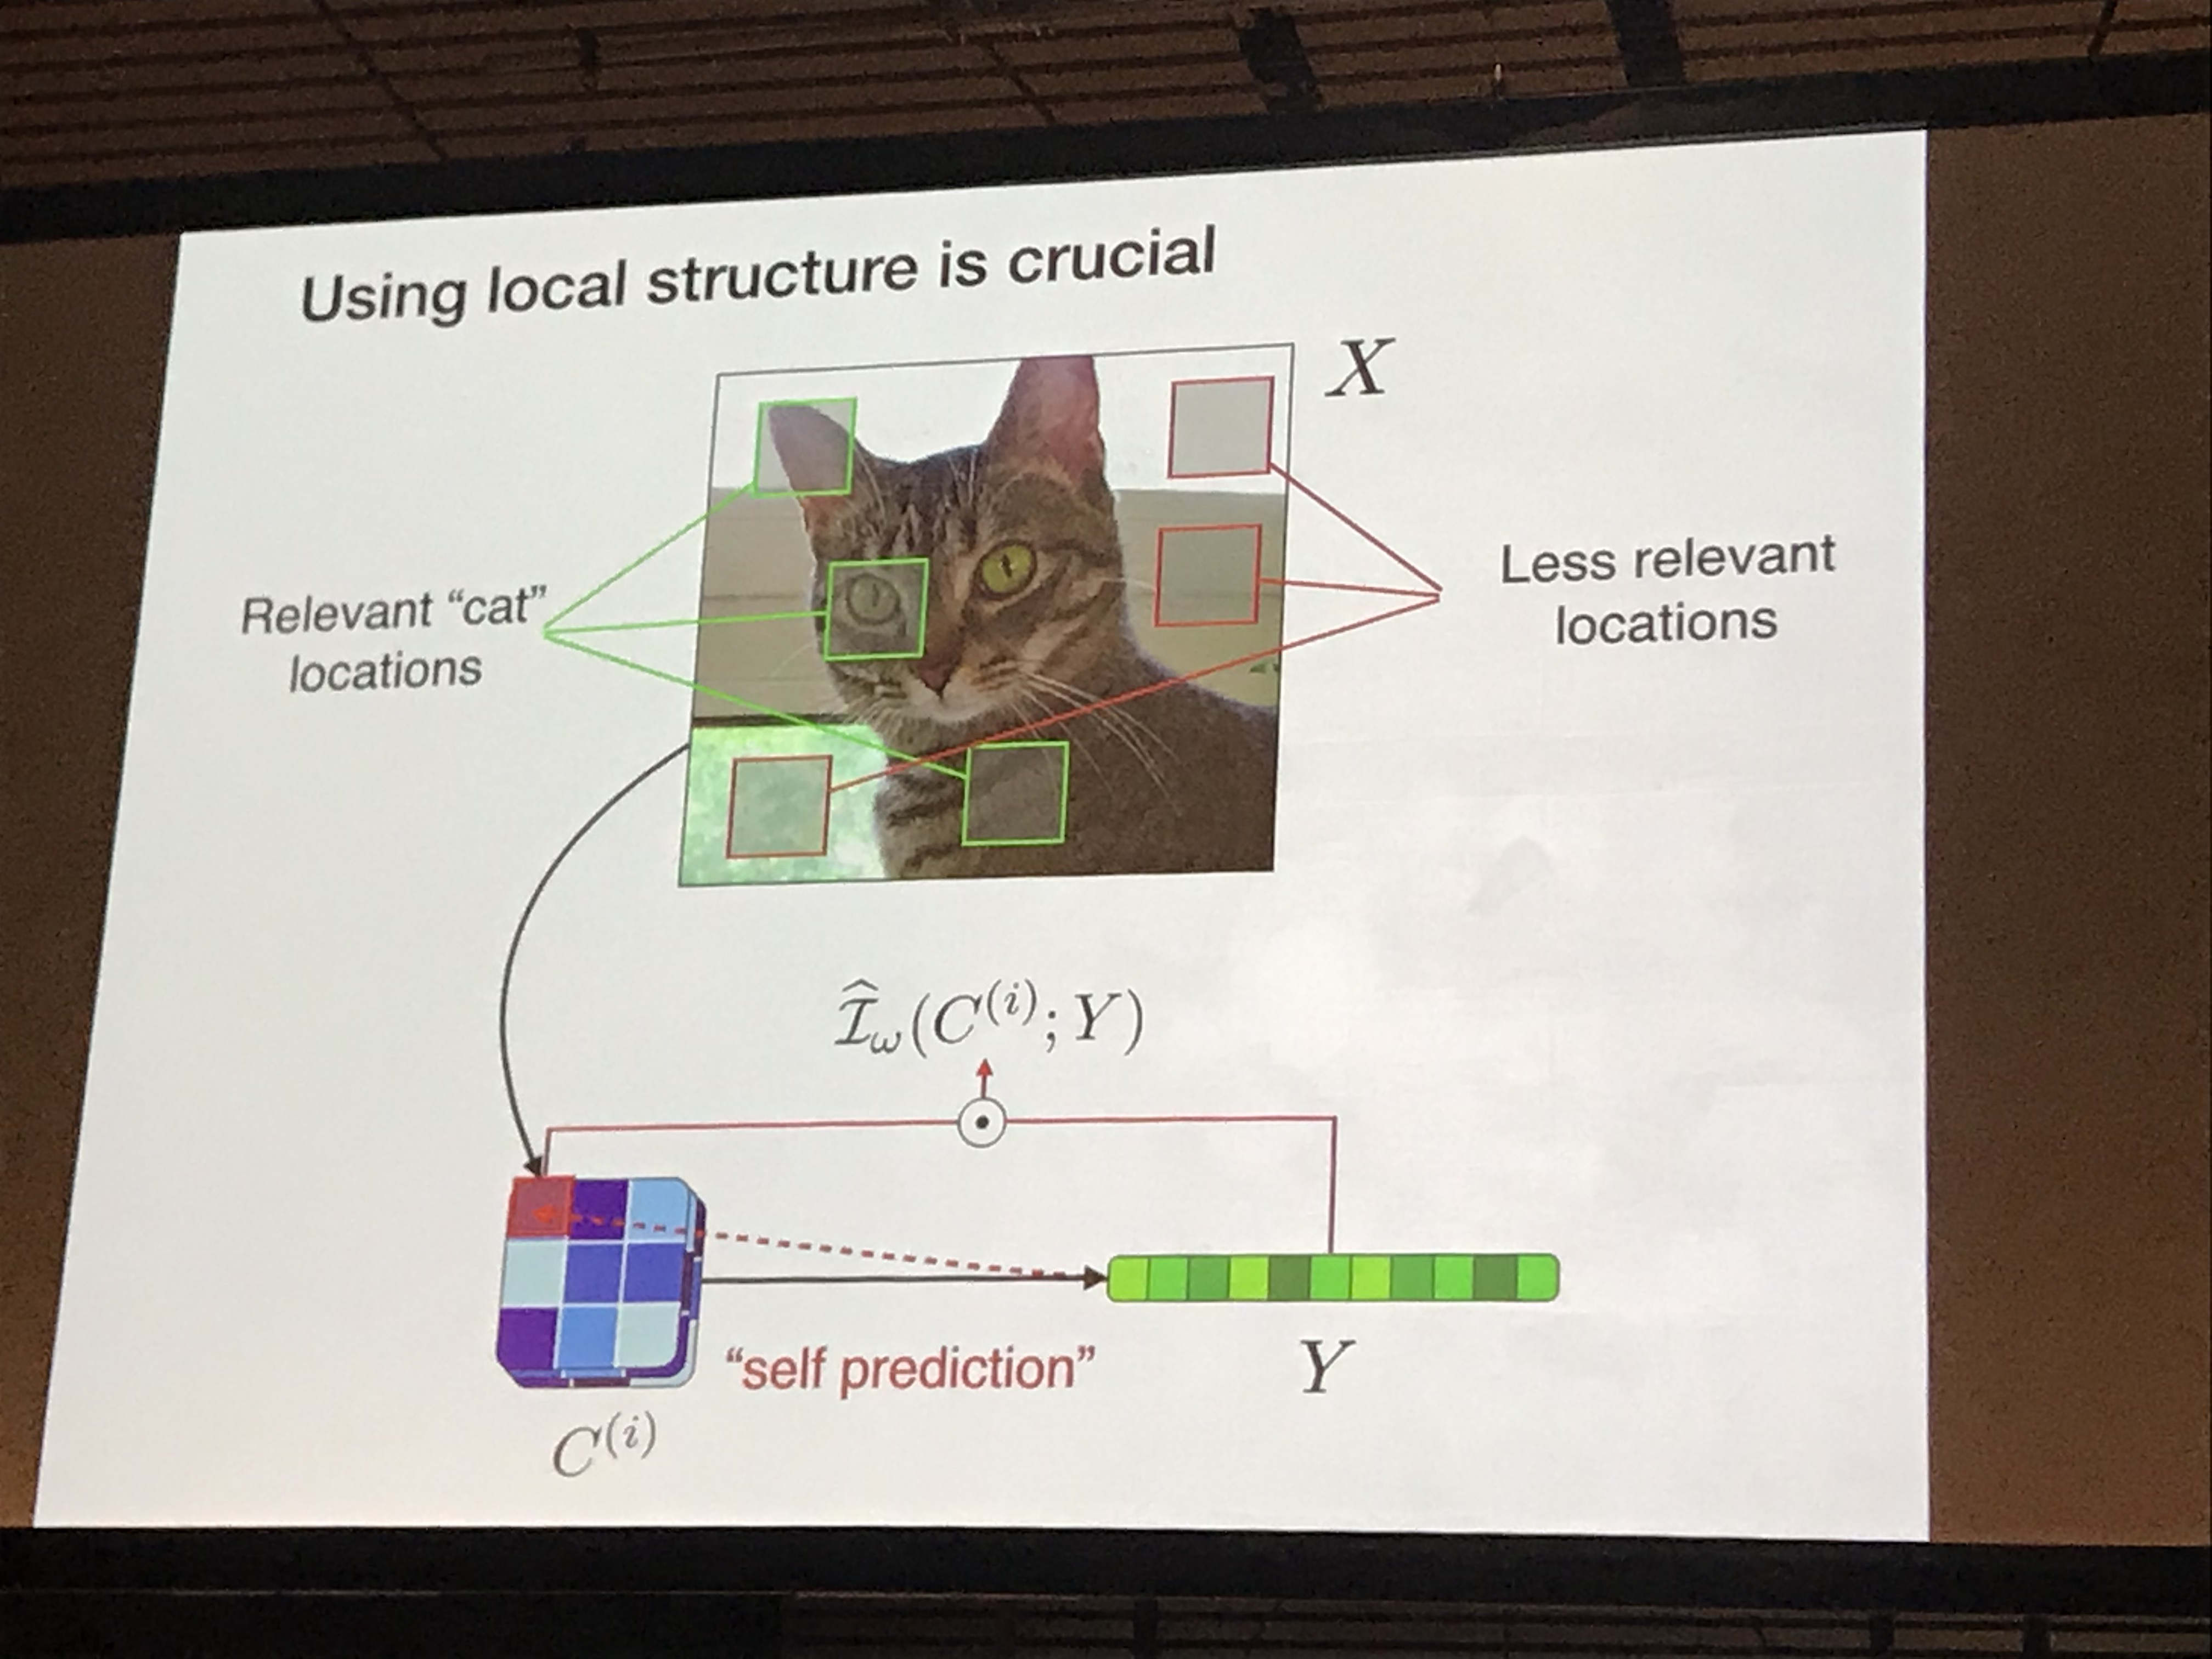
\includegraphics[width=0.4\textwidth]{images/cat.JPG}
    \caption{Extracing local feature maps via local mutual info estimation and maximization}
    \label{fig:cat}
\end{figure}

Evaluation: depends heavily on downstream task. Can measure mutual info, down stream performance on classification/regression tasks, and so on. \\

$\ra$ Deep Info Max performs very well when the learned representation is used in downstream tasks like classification. \\

Other tasks investigated: prior matching, coordinate prediction, relative coordinate prediction \\

\dnote{Off to more meetings.}

\subsection{Keynote: Zeynep Tufekci on Dangers if ML Works}

Grew up wanting to be a physicist! But: eventually, many physicist encounter the {\it nuclear} problem: massive ethical issues facing the advancement of a scientific field. \\

$\ra$ At CERN recently: giant projects! 700 people on the Higgs Boson paper. They were concerned about how to divide up the Nobel prize, meanwhile in CS we're worrying about the impact our tools have on society, security, labor, climate, social infrastructure, and beyond. So: lots of ethical issues in CS, too! \\

Back in Turkey: no internet, limited access to culture/TV from the outside world (grew up watching little house in the prairie). But, got internet connection through working at IBM. \\

$\ra$ Wonderful to have unimpeded access to lots of information and connections to people! Lots of optimism about the power for this tool to do good in the world \\


{\bf This Talk:} big dangers that we're sleepwalking into. Going to end up in a scary and unhappy place, we will end up having built and contributed to part of it. \\
\begin{itemize}
    \item Seven years ago: the ``cat" paper, that learned to recognize cats on YouTube. Was hard to even imagine the current state of the field back in 2012.
    \item What we need to worry about: what if it works? What are we really introducing into the world?
\end{itemize}


{\bf Themes:}
\begin{enumerate}
    \item You are part of this world, and your tools will be too.
    \item These tools won't be used the way you think they will be.
    \item Alternative paths are possible.
\end{enumerate}

\subsubsection{Examples Of Ways Things Can Go Wrong}

Example 1: social movements in the public sphere. Specifically, the Facebook news feed:
\begin{itemize}
    \item Optimized to keep people engaged on the website
    \item Recall: Ferguson, MZ, shooting of an african american teen by a police officer. Similarly: in a McDonalds, some customers were thrown into a van without any chance to say anything (by some police officers).
    
    $\ra$ Huge discussions about these events on Twitter, but {\it not} Facebook. 
    
    \item Point: Friends {\it were} talking about it, but these issues weren't ``engagement friendly" for Facebook (it was trying to populate news feed with things that would be liked/shared).
    
    $\ra$ At the time, the ALS ice bucket challenge was going as well. Very likeable/shareworthy, so that dominated most Facebook news feed.
    
    $\ra$ Chilling moment: icebucket challenge dominated the media/facebook as a result.
\end{itemize}

Difference for social movements isn't whether you hold a protest. The thing the movements manage to do to be most effective is get attention. \\

$\ra$ But our algorithms are optimized to keep people engaged, so it tends to not spread certain kinds of information. A new form of censorship. \\

{\bf Classic finding:} People that tend to be into one conspiracy theory tend to be into others (from social science). \\

$\ra$ Instagram would recommend similar conspiracy theories, not because designers recommend them, but just because the algorithm learned this social science fact (someone likes a ``faked moon landing" post will also be presented with tons of other conspiracy theories). \\

in 2016: these phenomena were {\it widespread}. Watching one certain kind of video would immediately bias future videos (if you watch a jogging video, it then leads you to hardcore marathon training, if you watch a vegetarian video, it then leads you to vegan videos). \\

{\bf Point:} YouTube algorithms tends to {\it lead individuals down more polarizing and extreme routes}. Not by hand-design, but it does it {\it to increase engagement}. \\

$\ra$ Hate speech, extreme views, and so on, are very ``shareworthy" and capable of improving engagement.

\subsubsection{ML and its Challenges}

Some core challenges of implementing ML systems in the world:
\begin{enumerate}
    \item Bias
    \item Interpretability
    \item Potency-at-scale Restructuring power
    \item Surveillance and Privacy
    \item Transition and Upheaval
\end{enumerate}

Example: suppose you're hiring, and suppose you use ML to hire. \\

(rhetorical) Q: We have methods for predicting depression rates; what if your ML system in using this information for hiring outcomes? \\

Problem: You won't even know that your system is using this information! \\

Similar problem: can use a ``mirror population" system (identify similar groups) to target individuals that are fear-prone with well designed ads to encourage voting for authoritarians? (again coming from findings in social science). \\

$\ra$ The way these systems are built {\it incentivizes} surveillance, since data about individuals/groups is always important. Data {\it will} get out, and will be used. \\

{\bf Path Forward:} build things that can do what we want to do, but not let it control us and be used on things we dont want it to be. \\

**We are in a very particular historic moment: all the companies here are trying to recruit you. If these companies that are trying to recruit you, but can't get you to do the things they want you to do, but you {\it insist} on using privacy-preserving methods. \\

{\bf Takeaway:} Lots of good the talent in this room can do. \\

Some thoughts:
\begin{enumerate}
    \item Google gave away money for ML projects. One of them was on detecting societal ideation, someone at risk, and do intervention.
    
    Seems like a great 
    
    \item What will happen: university will expel kids with mental health issues. They don't want that happening in their dorms.
    
    \item Look at the database of people killed by police officers. Many people are in a mental health crisis.
    
    $\ra$ Suicide detection program can be used in a very bad way (like laws that prevent at risk individuals from basic needs/goods).
    
    \item But! Imagine a privacy preserving system designed to help individuals instead.

\end{enumerate}

First earth day: pictures were blurry because of smog. Now that's not the case! So, a final note: genuinely consider unionizing. \\

Union: you get a huge number of legal protections. You get some freedom of speech. Organize your own industry ML group. \\

No one here is trying to explicitly go down this dark path. So many good people in this community! But the business model plus the world leads us to the wrong kinds of systems.

Final thoughts:
\begin{enumerate}
    \item Organize
    \item Build alternatives
    \item Insist on having a voice
\end{enumerate}

*What we want, when someone wants to have a phone/app, we're just doing a bad job of what China is doing (in terms of monitoring/surveilance) for the purpose of selling more stuff. \\

$\ra$ We need a real alternative. We need the conveniences and empowerment, we need an option that repsects us, that gives us early warning and intervention but not at the expensve of subjecting us to mass surveilance. \\

{\bf Final Example:} Before Diffie-Helman (public key crypto), we didn't have a way of sending a message without exchanging secret keys. 
\begin{itemize}
    \item They thought this was a terrible problem. Needed to give people a way to communicate and exchange info without having to exchange keys beforehand.
    
    \item All of public key crytography comes from that. Really important and invidual-empowering tool that has dramatically reshaped the state of the world.
    
    \item So: stock options are cool, but we should be thinking about developing tools like this for the next generation of technology.
\end{itemize}


\subsubsection{Q \& A}
%({\it Questions}) \\

Q: Could you comment on AI in the military? \\

A: War in 2019: any form of it is going to be terrible. Anything that makes it more convenient will make it even worse. Governments should be accountable to us. \\

Q: Feels a bit US centric -- any thoughts on the broader international perspective? \\

A: Remember the paper that can detect (claims to) detect secual orientation. Ugandan government has outlawed homosexuality, so we need to keep these things in mind. If we have better healthcare some of these issues will be less damaging. Fixing the politics makes some of these dangers less potent. Important for silicon valley not to be in this bubble. Everytime I go to SanFran now, every other table around me is talking about when stock options vest. Even if you're making great money but healthcare isn't there and your technology is used to keep people from getting hired, it's problematic. \\

Q: Question about the ``solutions" part, and refusing to build unethical software. Often we build small parts of a big thing, how do you predict what's going to be harmful? \\

A: First, that's why we should organize and unionize. Second, refusal is powerful but will only last so long. Real path forward is the alternative path: can't get out of oil without solar/wind energy. Surveillance and data economy is our oil economy, and it's cheap. But we can develop the solar equivalent here, and insist on these alternatives that we can embrace. Third, you all might be on the product side: I encourage you to find people on your security team and talk to them. They see the worst.  They can warn you how these things might be used in the worst possible way. \\

\dnote{They did the last three questions together}

Q: Lots of surveillance in the US, and strong culture against whistleblowers, too. Should people at ICLR take a bigger stand? \\

A: Yes absolutely speak out against that. Encourage and support whistleblowers in your own company. \\


Q: What are the real problems, and what specific things should we be avoiding? We've seen engineers stand up to people working on the army. We've talked about companies that sell ads at any cost. \\

A: If the data exists, it will be sold and used. Great challenge: we need to figure out how to do some of this without surveilance. That includes, expiration dates on data, operating on encrypted data (insights on aggregate, not individualized). Key thing is to kill the surveilance economy. We can't kill phones, since those empower us, but we need an alternative. 

Q: Any comments on healthcare solutions?  \\

A: Lots of things! Skin care diagnosis and other tools that are empowring. Need to figure out a new full stack trusted method that doesn't feed into the surveilance economy. No way we can collect all this data and work on this data and not have the powerful corporations and governments come for it. We need to stop the sureilance economy. 


\subsection{Debate led by Leslie Kaelbling}

The debaters are: Josh Tenenbaum (JT), Doina Precup (DP), Suchi Sara (SS), Jeff Clun (JC), with Leslie's comments as LPK. \\


LPK: We are interested in questions from the audience! The topic is on structure in learning. Each panelist will do some intros: \\

DP: I drew the short straw. I'm going to argue that a lot of what we need can and should be learned from data rather than come from priors. Especially in the context of generally purpose AI, rather than special purpose applications. In a special purpose application we should definitely use structure/priors, but in making general AI, we want our systems to learn from data. See: AlphaGo. First we used the specialized human version with some expert knowledge, but then the approach that ended up dominating was the one that used entirely data. \\

JT: Other extreme! I want to emphasize what you can build in. I, like Doina, am interested in general AI. I'm not against learning, but I'm really struck by how much systems like AlphaGo {\it don't} do. We have a general toolkit for building a specific kind of intelligence, but not general intelligence. Transferring to a different board size, for instance, would require retraining from nearly scratch. I'm interested in taking inspiration from the ways humans come into knowledge, like learning from the stage of a baby. In the universe the only case we have of learning from an early/scratch stage are human infants. We've learned so much, a bit contrary to some of the (bitter) lessons that some people have been drawing. The findings in cognitive science we find tell a different story: lots of inductive biases in human children. Also: the gazelle, learns to walk in the savannah very quickly or it will be eaten. Or think about a bird: the first time it falls out of a nest it has to fly. Human babies don't start off being able to walk, but before they can do those things, they develop objects, intuitive physics, schemes for defining goals, some notion of space, and so on. Exciting opportunity to take those kinds of core systems and learn how to devise and go beyond them. I would like to think about how we can take the right kind of machinery that include what we know how to do in RL and deep learning, but also what we know about symobolic reasoning and classical methods, so they know how to live in a world. \\

JC: This debate is usully framed as two extremes: 1) build in the right stuff, and 2) learn everything from scratch. I think there's a third alternative here, which is what I call AI generating algorithms: algorithms that can search for an AI agent that on the inner loop is very sample efficient (which come from the outer loop doing the right thing). It's a nice marriage between the two things. When you have a new problem you don't learn from scratch, you deploy this new agent. We know that can work (existence proof: Earth, this happened!). The algorithm is evolution, the inner loop is the human brain. This research direction isn't to say that the outer loop has to be evolution, could be something else like meta learning. If we want to make progress here: three pillars:
\begin{enumerate}
    \item Meta learn the architectures
    \item Meta learn the learning algortihms
    \item Automate effective learning environments (scaffolding)
\end{enumerate}
Clear trend in ML that we're aware of: hand designed systems that work okay will be surpassed by approaches that are wholly data driven/rely on big compute. If you believe in this trend, you should also believe that it can apply to the discovery of this machinery itself. So: what are the structures that allow for sample efficient general purpose learning? This may be the fastest path for us to pursue these big goals. \\

SS: I'm going to oversimplify a bit. Each of the three other panelists proposed a solution path, so I want to highlight some observations, first:

\begin{enumerate}
    \item Observation 1: Josh and Jeff suggested that if we want to build human-like intelligence, and we know we can get there during learning. Proof for this is evolution. Evolution is very slow. In the process of getting to us lots of calamities. So, a big issue:  we can't afford to make our civilization to go extinct or to make societal level mistakes. What does it mean for us to come up with the right paradigm since we can't afford to make mistakes?
    
    \item Observation 2; What are the levers we have in ML? Algorithms learn by interacting or from past data. So the question is: can we conclude that if we have data and interactions alone, we can learn anything we want? Unclear!
    
    \item Observation 3: As a field we focus very hard on incrementing on a solution set. I'm curious if we have answers to these kinds of questions: what can we learn easily, starting from a superintelligent being. Do we have a taxonomy for what's easy to learn what's hard to learn? Can we define where the gaps are? Might be good to define the strategy here!
\end{enumerate}

So, do we really want to be as slow as evolution or take into account what we know? Definitely the latter \\

\spacerule

LPK: Really important for us to each define our own objectives. We each have different big and small scale objectives. Big scale: understand math of learning, biology of the brain, making things work in 10 years or 100 years. So one reason to make this not a knockdown debate is that probably no answer will be true for every objective. So can you each say something more about your objective? \\

DP: I have multiple objectives. Want to understand how to build general AI agents. Some of the things we do now don't align with that goal: we often train from scratch, but don't necessarily need to do that! We could load a vision system in and learn downstream aspects. Would be great to emphasize this kind of continueal learning a bit more. Other chunk of my time I think about medical applications: it's a space where we don't have a lot of data and we can't always intervene because of ethical considerations. Here we often use structure/priors. Conceptual thing: what are the principles of intelligence? Focusing on learning from data can get us to that. People are wonderful but there are other intelligent things in nature too. Working on these algorithmic questions can help us understand much of nature. \\

SS: To me, the biggest challenge is how do we proceed when our objective is broken? (see previous keynote!) Lots of research is asking the right question. Who is going to define the question? How should we think about defining the right objective? \\

DP: That's true! We can have different objectives and that's okay. \\

JT: I'll say quickly: we're all pretty broad minded people but we have our strong deep views about things. I love the evolutionary view. We look at the learning algorithms we've seen, Evolution is the master algorithm (Pedro Domingos). Gazelles/animals are deeply fascinating. Also cultural evolution, especially once you have language, opens up whole new possibilities. The success of AI tools has in large part occurred due in part to the cultural evolution that lets us build collective knowledge and share goals and ideas. \\

JC: I'm interested in how to build intelligence piece-by-piece. But also interested in building a process that can build intelligent systems. Also fascinating to think about the set/space of possible intelligent entities. In part we're motivated by what looks like us, but we might miss out on huge regions of what intelligent/sentient systems look like. Also motivated by applications in healthcare, and beyond. Great opportunity for all of us! \\

LPK: Okay now we'll go to audience questions. This one is anonymous: ``What kind of results would cause you to change your opinion on how much structure vs learning is necessary?" --- How much structure is necessary is the wrong question? You can contextualize this with respect to a particular objective and get a really fascinating question. Hard to prove a negative. We're in the midst of a methodological crisis because we're all putting points in a space. Colleagues? \\

JT: I know one case study I find interesting about intuitive physics: being able to predict/imagine/plan to causally intervene on objects. All about predicting ``what happens if I hit this thing with that thing?". We built a system that didn't do any learning, just did probabilistic inference using a game engine. Other people around the same time tried tackling same problems but in an end-to-end learning method in some impressive ways. Still required huge amount of data and didn't seem to generalize to well. Others have been trying different systems. We've had some workshops on this topic, and reached broader argument: not an argument for necessity, but an empirical result. Building in some models of objects that might interact via contact/having close spatial locality is extremely powerful. We can't prove they're necessary but they're massively effective. Doesn't change any one person's mind but it's a case where we'ved learned some important empirical lessons that turn out to be valid. \\

DP: Can be very valuable to build these things in, but I'm not convinced that we can't just learn these things. The main complaint is usually sample complexity: if we had the right kind of approach for the learning algorithm it could learn these things. Typical example is causality. If we had the right learning algorithm we could learn a causal model not a predictive model. Another short thing about methodology, also very important for us as a field. Difficult to make progress when we care a lot about numbers without also understanding what our systems do. So yes it's great when our algorithms do better, but we need to also understand why. I want to argue that we need to probe our systems not just measure our systems quantiatively/qualitativey, but really probe our systems via hypothesis testing. \\

JC: I agree with Doina! Just wanted to ask Josh: might give us a big lift by building these things in, but perhaps we can learn even better lifts? How do you see things like HoG and SIFT where we eventually learned something better? \\

JT: Yeah, HOG and SIFT is a very instructive example. We see things in intuitive physics with a similar story: right now the best models we have are physics engines (for playing video games, for instance). But we know there's lots of things they don't capture. Recent work starting to learn physics simulators that can improve on these classical notions of physics simulators. We don't know where that story will end. If we look at vision, not just HOG and SIFT, you see the community over a few generations of research, we see the same motifs/ideas repeated (non-linearity, hierarchy, etc). Many versions of the same idea. HOG and SIFT were one idea, AlexNet was another. We'll see similar ideas recurr and build and call back to the same motifs. \\

SS: Josh, question for you: do you think the reason we need more than learning is that you think these systems cant be learned from scratch? Can we learn physics just by learning? \\

JT: That's what happened on Earth via evolution. Compute for simulating evolution is huge and we're just barely start to making progress. So the current route of modern deep RL is not necessarily going to deliver on this promise to learn an entire physical model. Human children are proof that some other route works. \\

JC: I think lots of routes can get to general AI, but it's partially a question of which is the fastest route. It's an open question as to whether the manual path will get there faster than the meta learning or evolutionary approach. \\

SS: Except you missed this along the way: what about everything that happens along the way? \\

JC: Fascinating question! General question of whether we should be building a general AI? Also, what should we be doing along the way to building that? Very real considerations. What's the fastest way to get there: I say the meta-learning approach above. Regarding ethics? Lots of open questions, too. \\

LPJ: One thing Jeff didn't mention was the physical infrastructure required to make this work. Robots need to interact with the world unless we rely on a perfect simulator. I'm not sure we can get that taking off that we might suggest.

\spacerule

LPK: Next question ``Symbol manipulation has no place in deep learning. Change my mind" (Yann LeCun). Symbol means something different to embody; I'd argue that embeddings are roughly symbol manipulations, so maybe you've been doing it and you don't actually know. \\

JT: Certainly not my place to define what deep learning is. One reason it's interesting is that deep learning can mean a lot of things; it could mean and already sort of does mean doing SGD and symbol manipulation. Nice talk tomorrow on this. Whole community trying to explore interesting ways for symbols to live inside of systems that do deep representation learning. Multiple ways to learn a representation, might include symbols or combinations of these. We'll see systems that do things better than without these different techniques. \\

DP: But will we see systems that do this from scratch? \\

JT: Having a basic path for compositionality that gives us meaning/function that wasn't there from the beginning. \\

DP: Meaning as in people assign meaning? Or meaning as in what the machine defines for itself? \\

JT: Whatever you mean! ... If we want to build systems that we trust that we think do have the right kind of meaning, it's one reason to build AI that have these kinds of structure/symbols. \\

\spacerule

LPK: Q from Yoshua Bengio: ``We of course need priors but to obtain the most general AI, we'd like the least amount of priors which buy us the most towards AI-tasks, don't we?" \\

JC: Yes! \\

SS: Also yes, New question for the audience: everything can be learned? (some hands) not everything can be learned (more hands) -- some examples from audience poll of things that can't be learned: causality, halting problem, false things. \\

\dnote{Need to run out for a meeting! Fantastic debate though.}